% FCSG-Net B.Tech research project report, SHORT version (about 30 pages).
% The full version is main.tex; both share FrontPages.tex, macros and Ref/.
% Built on the NIT Rourkela DissertationGuidelinesV4_5 template (copy kept in
% college_reference/). Needs the college bundle files listed in thesis/README.md
% (NITR.cls, FrontPages.tex, Ref/*.bst) before it will compile.
\documentclass[12pt,a4paper,oneside]{NITR}

\usepackage[hyphens]{url}
\usepackage[none]{hyphenat}
\usepackage{amsmath,amsfonts,mathdots,amssymb}  % template also loads yfonts (blackletter), unused here
\usepackage{graphicx}
\usepackage{xcolor}
\usepackage{tikz}
\usetikzlibrary{trees,shapes}
\usepackage{booktabs}
\usepackage{multirow}
\usepackage{longtable}
\usepackage{subcaption}
\usepackage{siunitx}            % aligned decimals in result tables
\sisetup{group-separator={,},group-minimum-digits=4}

% Report figures are already generated as vector PDFs by
% evaluation/build_technical_report.py. Reference them in place, do not copy.
\graphicspath{{figures/}{../output/pdf/fcsg-report-assets/}{../results/diagnostics/}}

% Shared macros. Keep this file small.

% Writer notes. Every \todo prints in red so nothing ships half-written.
% Before final submission: grep -rn '\\todo' thesis/ must return nothing.
\newcommand{\todo}[1]{\textcolor{red}{\textbf{[TODO:} #1\textbf{]}}}
% Where a number came from. Renders nothing, exists for reviewers of the .tex.
\newcommand{\evidence}[1]{}

\newcommand{\fcsg}{FCSG-Net}
\newcommand{\dB}{\,dB}
\newcommand{\expert}[1]{$E_{#1\times#1}$}   % \expert{7} -> E_{7x7}


\onehalfspacing
\begin{document}
\sloppy
% ---------------------------------------------------------------- front matter
% ======================================================================
% Front-page fields. STAND-IN layout: when the college FrontPages.tex
% arrives, copy these values into its fields and replace this file.
% ======================================================================
\reportTitle{FCSG-Net: Frequency-Band Spatial Expert Routing\\for Lightweight Composite Image Restoration}
\docType{Project Report}
\degree{Bachelor of Technology}
\dept{Computer Science and Engineering}
% Ascending order of roll number.
\authors{Akshat Mittal (123CS0954)\\Risav Rathi (123CS0957)\\Ramnath Thakur (123CS0965)}
\authorsInline{Akshat Mittal (123CS0954), Risav Rathi (123CS0957) and Ramnath Thakur (123CS0965)}
\newcommand{\supname}{Dr.\ Shyampada Mukherjee}
\supervisorOne{\supname}
\submitDate{November 2026}

\ackText{%
We thank our supervisor, \supname, for guiding us through this project.

We thank the Department of Computer Science and Engineering, National
Institute of Technology Rourkela, for the chance to do this work. Kaggle
gave us free GPU time. Without it we could not have trained four models for
200,000 updates each.

We thank the DIV2K authors for making their dataset public. We also thank
Kai Zhang and colleagues for releasing the FFDNet code and pretrained
weights, which let us check our implementation against a published result.

Last, we thank our families and friends for their patience and support.
}

\abstractText{%
Old photographs usually carry several kinds of damage at once. Optical blur,
lost resolution, sensor or film noise and lossy JPEG compression each hit a
different part of the image spectrum. We ask whether a very small
restoration network can make use of that. Our network, FCSG-Net, splits the
degraded image into low, mid and high frequency bands with fixed, soft radial
masks in the Fourier domain. Three shared convolutional experts, with
$7\times7$, $5\times5$ and $3\times3$ kernels, process every band. A small
gate picks the two best experts for each band at every pixel. The model has
97,088 parameters and costs 9.39 GFLOPs for a $256\times256$ input. We first
verified the implementation and reproduced the published FFDNet result to
within 0.01\,dB. We then trained FCSG-Net, DnCNN and two FFDNet variants from
scratch on the same synthetic composite degradation of DIV2K images, with one
schedule and one evaluation protocol. On 100 validation images FCSG-Net
reaches 27.24\,dB PSNR. DnCNN reaches 27.83\,dB and blind FFDNet 28.19\,dB,
and FCSG-Net uses 82.6\% fewer parameters than DnCNN. The low FLOP count did
not make it fast. On a Tesla T4 GPU it is the slowest of the four. The
learned routing varies across the image and follows the noise level, with
within-image correlations up to 0.81. Overriding the gate's choices at
inference costs 0.37\,dB on average. Frequency-band routing gives a small
model behaviour we can inspect. Within this budget, it does not make the
model more accurate or faster than simple convolutional baselines.
}

\keywords{image restoration, frequency decomposition, mixture of experts,
spatial routing, lightweight networks}
            % college file: title, names, roll nos, guide(s)

\coverPage
\titlePage
\certificateOfExamination

\certificateOneSupervisor
%\certificateTwoSupervisors

%\dedication                    % add \dedicationText in FrontPages.tex to use
\declaration
\acknowledgment
\abstract

\tableofcontents
\cleardoublepage
\addcontentsline{toc}{chapter}{List of Figures}
\listoffigures
\cleardoublepage
\addcontentsline{toc}{chapter}{List of Tables}
\listoftables
\cleardoublepage

% ---------------------------------------------------------------- main matter
\pagenumbering{arabic}
\pagestyle{fancy}
\renewcommand{\chaptermark}[1]{\markboth{#1}{}}
\renewcommand{\sectionmark}[1]{\markright{\textbf{Chapter \thechapter}}}

\chapter{Introduction}\label{ch:intro}

\section{Motivation and problem}\label{sec:motivation}

An old photograph is rarely damaged in just one way. A print shot through a
soft lens on grainy film, scanned at low resolution and saved as a
compressed JPEG carries all of those defects, and each one hits a different
part of the spectrum. Blur removes high frequencies. Resampling throws away
detail above a resolution limit. Noise dominates where the signal is weak,
which in natural images means the high frequencies. JPEG quantises the mid
and high frequencies of each $8\times8$ block. Most restoration networks
treat the mixture as a single problem, and the strongest of them, such as
Restormer \cite{zamir2022restormer}, need tens of millions of parameters.

We ask whether a very small network can use this spectral structure
directly. It splits the image into frequency bands, and a learned gate
chooses between convolutional experts of different kernel sizes for every
band and every pixel. We call the network \fcsg{}.

Formally, we degrade a clean RGB image $f\in[0,1]^{H\times W\times 3}$ as
$x=\mathcal{D}(f;\theta)$ with $\theta=(\sigma_\text{blur}, s, \sigma_n, q)$.
$\mathcal{D}$ applies Gaussian blur, bicubic down- and up-sampling by $s$,
Gaussian noise with standard deviation $\sigma_n$, and JPEG at quality $q$.
We draw the parameters at random for each image and hide them from the
model. We want $\hat f=g_\phi(x)$ close to $f$ in PSNR, SSIM and LPIPS, with
fewer than five million parameters and fewer than ten GFLOPs for a
$256\times256$ input.

\section{Objectives and contributions}\label{sec:objectives}

We test one hypothesis. \emph{Apply a fixed frequency decomposition, then
route each band per pixel to the top two of several shared kernel-size
experts. The routing will change with content and degradation, and the
trained network will depend on it, all within the budget.} The work has four
objectives.
\begin{enumerate}
	\item[\textbf{O1}] Build \fcsg{} and verify it before training.
	\item[\textbf{O2}] Get trustworthy baselines by reproducing a published
	FFDNet result.
	\item[\textbf{O3}] Compare \fcsg{}, DnCNN and two FFDNet variants trained
	under one matched protocol, in quality, size and measured speed.
	\item[\textbf{O4}] Describe what the router learned.
\end{enumerate}

We contribute a 97,088-parameter network with its verification suite, a
matched composite-degradation benchmark, and a routing analysis that links
expert weights to the recorded degradation. We also report the outcome as it
is. \fcsg{} comes within 0.6\dB{} of DnCNN with 5.7 times fewer parameters,
but it is not faster on a GPU. We claim neither state-of-the-art quality nor
novelty, since frequency decomposition and expert routing both have a long
history (Chapter~\ref{ch:literature}).

Chapter~\ref{ch:literature} reviews related work and
Chapter~\ref{ch:method} describes the method. Chapter~\ref{ch:setup} covers
the experimental setup and verification. Chapter~\ref{ch:results} gives the
results and the routing analysis, and Chapter~\ref{ch:conclusion} concludes.

\chapter{Related Work}\label{ch:literature}

Published scores from the works below use other tasks, datasets or noise
protocols, so they serve only as context. Our result tables contain only
models we trained and evaluated ourselves.

\paragraph{CNN restoration.} DnCNN \cite{zhang2017dncnn} showed that a deep
stack of convolutions with batch normalisation learns denoising much more
easily by predicting the noise residual. FFDNet \cite{zhang2018ffdnet}
processes four half-resolution sub-images and takes a noise-level map as an
extra input, so one network covers a range of noise strengths; the author's
colour model has 852,108 parameters and reports 31.21\dB{} on CBSD68 at
$\sigma=25$. Its map describes only Gaussian noise, not blur or JPEG. Larger
transformer-based restorers reach higher quality but need tens of millions of
parameters, far outside our budget.

\paragraph{Frequency-domain restoration.} MWCNN \cite{liu2018mwcnn} replaces
pooling in a U-Net with wavelet transforms and processes subbands jointly,
which motivates our cross-band fusion. The closest work is SFNet
\cite{cui2023sfnet}, which already performs local, content-adaptive frequency
selection inside a U-shaped network. Our distinction is narrower: \fcsg{}
uses \emph{fixed} radial masks and puts the learned spatial decision in the
choice among shared $7\times7$, $5\times5$ and $3\times3$ experts, which we
can then compare with known degradation parameters.

\paragraph{Mixture of experts.} Shazeer et al.\ \cite{shazeer2017moe} route
each example to a few experts with a top-$k$ gate and balance load with
auxiliary penalties. The efficiency argument for sparse experts depends on
not running the unselected ones. Our implementation computes every expert and
mixes them with sparse weights, so sparsity here aids analysis, not speed.

\paragraph{Metrics.} PSNR is $10\log_{10}(1/\mathrm{MSE})$ on $[0,1]$ RGB
images, computed per image and averaged. SSIM compares local means, variances
and covariances in an $11\times11$ Gaussian window ($\sigma=1.5$). LPIPS
\cite{zhang2018lpips} measures distance between deep features (AlexNet
variant); lower is better, and it can disagree with PSNR.

Table~\ref{tab:gap} summarises the positioning. Each ingredient of \fcsg{} is
established; the project studies one combination of them under a tight
budget.

\begin{table}[htbp]
	\centering
	\caption{Positioning of \fcsg{} against closely related methods.}
	\label{tab:gap}
	\small
	\begin{tabular}{@{}lcccl@{}}
		\toprule
		Method & Freq.\ split & Learned selection & Spatial & Notes \\
		\midrule
		DnCNN \cite{zhang2017dncnn}      & --         & --              & --        & residual CNN \\
		FFDNet \cite{zhang2018ffdnet}    & --         & --              & --        & noise-map input \\
		MWCNN \cite{liu2018mwcnn}        & wavelet    & --              & --        & joint subbands \\
		SFNet \cite{cui2023sfnet}        & learned    & frequency       & local     & closest prior work \\
		Sparse MoE \cite{shazeer2017moe} & --         & experts         & --        & per-example routing \\
		\fcsg{} (ours)                   & radial FFT & experts, top-2  & per pixel & 97k parameters \\
		\bottomrule
	\end{tabular}
\end{table}

\chapter{Proposed method: \fcsg}\label{ch:method}

\section{Degradation model}\label{sec:degradation}

Our synthetic pipeline applies four operations in physical order
(Table~\ref{tab:degradation}). We quantise the image to 8 bits before the
blur and again before JPEG encoding. Each sample stores its parameters. The
network never sees them, but we use them to analyse the routing in
Section~\ref{sec:routing}. The mean input PSNR on our validation set is
20.99\dB{}.

\begin{table}[htbp]
	\centering
	\caption{Composite degradation, sampled independently for every image.}
	\label{tab:degradation}
	\small
	\begin{tabular}{@{}lll@{}}
		\toprule
		Stage & Parameter & Distribution \\
		\midrule
		Gaussian blur        & $\sigma_\text{blur}$ & $\mathcal{U}(0.5,\, 2.0)$ pixels \\
		Down/up resampling   & scale $s$            & $\mathcal{U}(1.0,\, 2.0)$, bicubic \\
		Additive noise       & $\sigma_n$           & $\mathcal{U}(5,\, 50)/255$, clipped \\
		JPEG compression     & quality $q$          & integer in $\{30,\dots,95\}$, 4:4:4 \\
		\bottomrule
	\end{tabular}
\end{table}

\section{Architecture}\label{sec:arch}

The network splits the input into low, mid and high frequency bands, and
each band is an ordinary RGB image. Three shared experts $E_7,E_5,E_3$
process every band. A spatial gate gives each expert a weight for every band
and pixel and keeps the top two (Figure~\ref{fig:architecture}):
\begin{align}
	y_b(u,v) &= \textstyle\sum_{e} w_{b,e}(u,v)\, E_e(x_b)(u,v), \qquad b\in\{L,M,H\},\label{eq:mix}\\
	\hat f &= x + \mathrm{Refine}\big(\mathrm{SEFusion}([y_L,y_M,y_H])\big).\label{eq:out}
\end{align}

\begin{figure}[htbp]
	\centering
	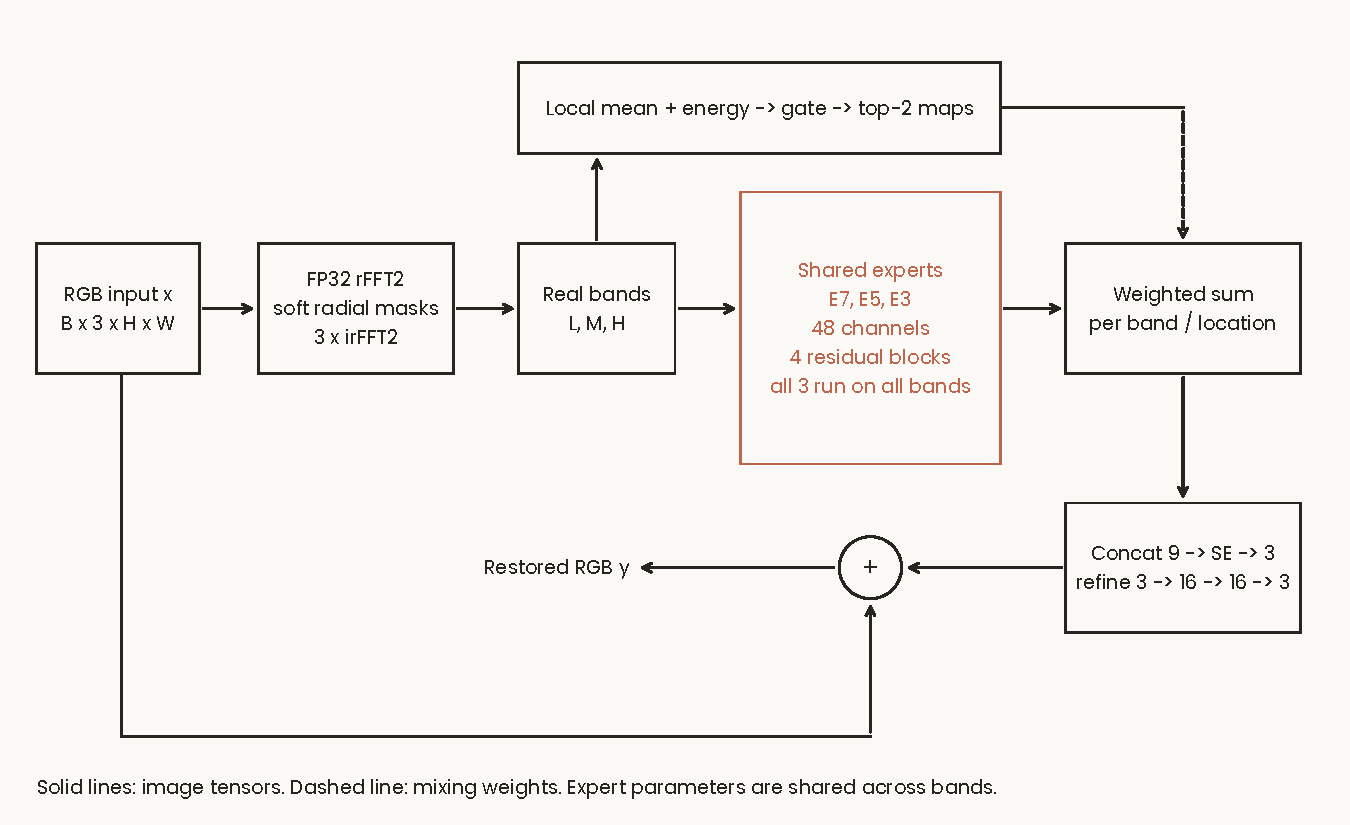
\includegraphics[width=0.95\linewidth]{architecture.pdf}
	\caption{\fcsg{} data flow. The bands share expert parameters.}
	\label{fig:architecture}
\end{figure}

\paragraph{Frequency decomposition.} Let $X$ be the orthonormal real FFT of
$x$ and $r$ the radial frequency in cycles per pixel. A soft low-pass mask
with cutoff $c$ and width $\Delta=0.05$ is
$\mathrm{LP}_c(r)=\tfrac12\big(1+\cos(\pi\,\mathrm{clip}((r-c)/\Delta+\tfrac12,0,1))\big)$.
With $r_1=0.10$ and $r_2=0.25$ the band masks are $M_L=\mathrm{LP}_{r_1}$,
$M_M=\mathrm{LP}_{r_2}-\mathrm{LP}_{r_1}$ and $M_H=1-\mathrm{LP}_{r_2}$, and
$x_b=\mathcal{F}^{-1}(M_b X)$. Three choices matter here. The masks sum to
one, so $x_L+x_M+x_H=x$ exactly. The cutoffs are normalised frequencies, not
FFT bin indices, so a band means the same thing on a $128\times128$ training
crop as on a full image. And each band goes back to the spatial domain before
any learned layer. A convolution over a spectrum has no clear meaning, and
complex inputs make training unstable, so the experts stay plain real-valued
CNNs.

\paragraph{Experts.} Each expert starts with a $2\times2$ pixel unshuffle
\cite{shi2016espcn}, giving 12 channels at half resolution. A $1\times1$
convolution widens these to 48 channels. Four residual blocks follow, each
with two depthwise-separable stages \cite{chollet2017xception} of kernel
$k\in\{7,5,3\}$. A $1\times1$ tail adds back the unshuffled input, and a pixel
shuffle restores full resolution. Separable convolutions at half resolution
are what fit nine expert passes inside the compute budget. We name the
experts by kernel size only, because we have no evidence of what each one
specialises in.

\paragraph{Spatial top-2 gate.} A gate that decided once per image would be
a lookup table, and it would tend to settle on a constant choice. Our gate
pools the mean and the mean of squares of the nine band channels in
$16\times16$ windows. An $18\to24\to9$ network maps these 18 statistics to
one logit per band and expert, and the logits are upsampled to full
resolution. At each pixel the gate keeps the two largest logits per band and
normalises them with a softmax. The third expert gets zero weight. The loss
uses the dense softmax $p_{b,e}$ over all three. The gate has 681 parameters.
The network still computes every expert before mixing.

\paragraph{Fusion and refinement.} The nine band channels go through a
squeeze-and-excitation block \cite{hu2018se}, a $1\times1$ projection to RGB
and three $3\times3$ convolutions ($3\to16\to16\to3$). The output is a
residual added to the input, as in DnCNN.

\section{Training objective}\label{sec:loss}

\begin{equation}
	\mathcal{L}=\mathcal{L}_\text{char}+0.05\,\mathcal{L}_\text{freq}+\lambda_\text{ent}(t)\,\mathcal{L}_\text{ent}.
\end{equation}
The Charbonnier loss \cite{charbonnier1994} is
$\mathcal{L}_\text{char}=\operatorname{mean}\sqrt{(\hat f-f)^2+\varepsilon^2}$
with $\varepsilon=10^{-3}$. $\mathcal{L}_\text{freq}$ is the mean absolute FFT
of the error, which weights all frequencies equally.
$\mathcal{L}_\text{ent}=\sum_b\operatorname{mean}\sum_e p_{b,e}\log p_{b,e}$
is the negative routing entropy. Minimising it keeps all experts in use early
on. Its coefficient decays linearly from 0.01 to 0, which leaves the gate
free to commit by the end. The baselines use the same loss without the
entropy term.

\section{Size and compute}\label{sec:size}

\fcsg{} has 97,088 parameters. The $7\times7$, $5\times5$ and $3\times3$
experts hold 39,228, 30,012 and 23,868. The gate has 681, fusion 96 and
refinement 3,203. We count each multiply-accumulate as two FLOPs and add an
estimate for the FFTs. A $256\times256$ pass then costs 4.66 GMACs, or 9.39
GFLOPs, inside the limit. Section~\ref{sec:cost} shows that this count
predicted running time badly.

\chapter{Experimental setup}\label{ch:setup}

\section{Data, baselines and training}\label{sec:training}

We use DIV2K \cite{agustsson2017div2k}, with 800 training images and 100
validation images. Every reported result comes from the validation images.
Training reads from a cache of 32 fixed $128\times128$ crops per training
image, 25,600 tiles in all, with random flips and rotations. The degradation
runs on the fly, so each epoch sees new corruptions. For reproducibility we
also exported a fixed set of 5,000 pairs generated with seed 1234.

The baselines are an RGB DnCNN (17 layers, width 64, 558,403 parameters) and
FFDNet in the author's colour configuration (852,108 parameters), in two
variants. \emph{Oracle} FFDNet gets the true sampled noise level. No real
user would have that, so it serves as an upper reference. \emph{Blind}
FFDNet gets a constant map of $27.5/255$ and sees exactly what the other
models see. We train all four from scratch with the same settings
(Table~\ref{tab:hparams}). Each model trained once with an unfixed seed, on a
Tesla T4 in Kaggle sessions that resume from checkpoints.

\begin{table}[htbp]
	\centering
	\caption{Training configuration, the same for every method.}
	\label{tab:hparams}
	\small
	\begin{tabular}{@{}ll@{}}
		\toprule
		Setting & Value \\
		\midrule
		Optimiser and schedule & AdamW \cite{loshchilov2019adamw}, $2\times10^{-4}$ cosine \cite{loshchilov2017sgdr} to $10^{-6}$ \\
		Updates and batch      & 200,000; 16 crops of $128\times128$ \\
		Loss                   & $\mathcal{L}_\text{char}+0.05\,\mathcal{L}_\text{freq}$ (+ entropy for \fcsg{}) \\
		Precision              & FP16 mixed precision \cite{micikevicius2018amp} \\
		Hardware               & NVIDIA Tesla T4 (Kaggle) \\
		\bottomrule
	\end{tabular}
\end{table}

\section{Evaluation protocol}\label{sec:evalproto}

We degrade each of the 100 validation images once, with its index as the
seed, so all models see identical inputs. Inference runs on $256\times256$
tiles with 32 pixels of overlap, averaged where tiles meet. During training
we monitored PSNR on 16 fixed crops. That number does not compare with
full-image results. For \fcsg{} it is 30.59\dB{} on crops and 27.24\dB{} on
full images.

\section{Verification and baseline reproduction}\label{sec:verification}

Before training, a notebook on the same T4 ran the checks in
Table~\ref{tab:gates} and stopped at the first failure. The overfit check
earns its place. If a model cannot memorise one image in 200 steps it has a
bug, and finding that out in seconds beats finding it after ten hours of
training.

\begin{table}[htbp]
	\centering
	\caption{Checks run before training.}
	\label{tab:gates}
	\small
	\begin{tabular}{@{}lll@{}}
		\toprule
		Check & Criterion & Measured \\
		\midrule
		FFDNet weights, CBSD68 $\sigma{=}25$ & within 0.5\dB{} of 31.21 & 31.220\dB \\
		Band reconstruction & $x_L{+}x_M{+}x_H = x$ & max error $6.0\times10^{-7}$ \\
		Parameters / GFLOPs at $256^2$ & $<5$M / $<10$ & 97,088 / 9.39 \\
		Memory, forward + backward & $< 4$ GB & 0.60 GB \\
		One-image overfit, 200 steps & MSE $<0.01$, $<\frac14$ initial & ratio 0.18 \\
		Checkpoint restore, reproducible data & identical & passed \\
		\bottomrule
	\end{tabular}
\end{table}

To check our FFDNet code against a published number, we ran the author's
pretrained colour weights \cite{kair} on the 68 CBSD68 images
\cite{martin2001bsd} with the author's protocol. We got 31.220\dB{} against
31.21\dB{} in the paper, a gap of 0.01\dB{}. To test the training loop end to
end, we trained DnCNN on clipped Gaussian noise at $\sigma=25$. It reached
32.65\dB{} on DIV2K validation and 31.04\dB{} on CBSD68.

\chapter{Results and analysis}\label{ch:results}

\section{Restoration quality}\label{sec:main-table}

Table~\ref{tab:main} gives the main result on the 100 validation images.

\begin{table}[htbp]
	\centering
	\caption{Composite restoration on 100 DIV2K validation images after
	200,000 updates (input PSNR 20.992\dB{}). GFLOPs at $256\times256$.}
	\label{tab:main}
	\small
	\begin{tabular}{@{}lrrrrr@{}}
		\toprule
		Method & PSNR$\uparrow$ & SSIM$\uparrow$ & LPIPS$\downarrow$ & Params & GFLOPs \\
		\midrule
		DnCNN                     & 27.831 & 0.7795 & 0.3242 & 558,403 & 73.43 \\
		FFDNet, blind             & 28.190 & 0.7899 & 0.3176 & 852,108 & 27.89 \\
		FFDNet, oracle$^\dagger$  & 28.240 & 0.7920 & 0.3162 & 852,108 & 27.89 \\
		\fcsg{}                   & 27.243 & 0.7529 & 0.3961 &  97,088 &  9.39 \\
		\bottomrule
		\multicolumn{6}{@{}l}{\footnotesize $^\dagger$Receives the true noise level. An upper reference.}
	\end{tabular}
\end{table}

\fcsg{} lifts the input by 6.25\dB{}, yet it is the weakest model on all
three metrics. It trails DnCNN by 0.59\dB{} and blind FFDNet by 0.95\dB{},
and the LPIPS gap is wider still. It gets there with 82.6\% fewer parameters
and 87.2\% fewer reported FLOPs than DnCNN, and with 88.6\% fewer parameters
and 66.3\% fewer FLOPs than FFDNet. A few bad images do not explain the
shortfall. Both FFDNet variants beat \fcsg{} on all 100 images, and DnCNN
beats it on 93. On the six images where \fcsg{} beats DnCNN, it wins by up to
2.07\dB{}, so the two designs fail in different places.

Blind FFDNet is the strongest fair model even though its noise map is
constant. Its lead must come from the architecture, not from noise
conditioning. The oracle map adds only 0.05\dB{}, because noise is one
corruption out of four. All validation curves had levelled off by 200,000
updates, so nothing suggests longer training would close the gap.
Figure~\ref{fig:qual} shows an example restoration.

\begin{figure}[htbp]
	\centering
	\begin{subfigure}{\linewidth}
		\centering
		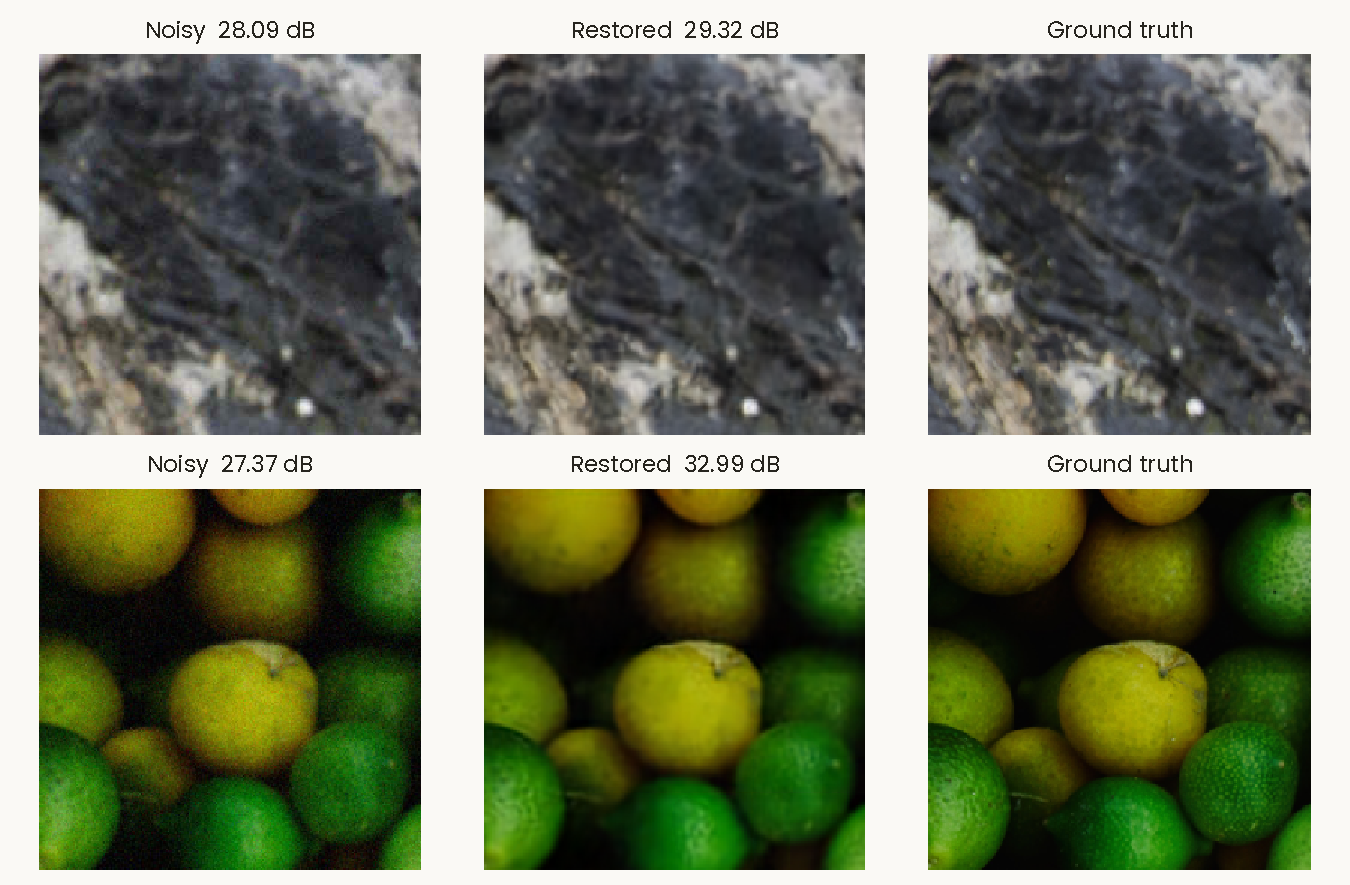
\includegraphics[width=0.85\linewidth]{qualitative_fcsg.pdf}
		\caption{\fcsg{}}
	\end{subfigure}\\[1ex]
	\begin{subfigure}{\linewidth}
		\centering
		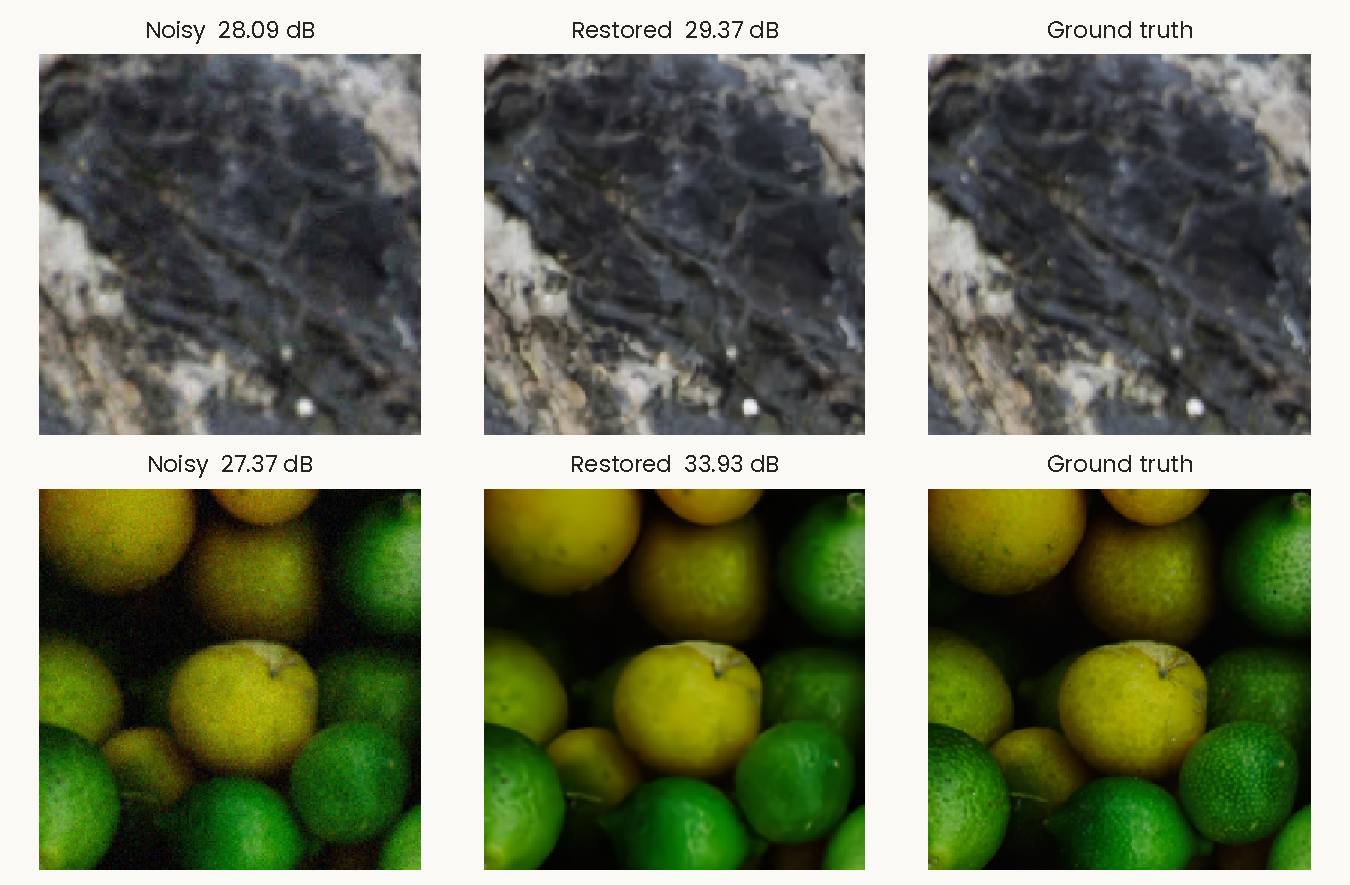
\includegraphics[width=0.85\linewidth]{qualitative_blind.pdf}
		\caption{FFDNet, blind}
	\end{subfigure}
	\caption{Degraded input, restoration and clean target on validation images
	0801 and 0802. The panels show the top-left $320\times320$ region. PSNR is
	for the whole image.}
	\label{fig:qual}
\end{figure}

\section{Computational cost}\label{sec:cost}

Table~\ref{tab:latency} gives the median FP32 forward latency at batch 1 on a
Tesla T4, measured after warm-up.

\begin{table}[htbp]
	\centering
	\caption{Median forward latency (ms) and peak inference memory at $256^2$ (Tesla T4, FP32).}
	\label{tab:latency}
	\small
	\begin{tabular}{@{}lrrrr@{}}
		\toprule
		Method & $128^2$ & $256^2$ & $512^2$ & Peak MB \\
		\midrule
		\fcsg{}          & 5.10 & 19.40 & 75.59 & 51.3 \\
		DnCNN            & 4.22 & 18.04 & 72.47 & 37.8 \\
		FFDNet, blind    & 1.69 &  6.30 & 24.12 & 20.2 \\
		\bottomrule
	\end{tabular}
\end{table}

\fcsg{} needs an eighth of DnCNN's FLOPs and a third of FFDNet's, and it is
still the slowest model at every size, with the highest memory use. Training
told the same story, at 5.84 steps per second against 9.41 for DnCNN and
26.67 for FFDNet. We did not profile individual operators, so our
explanation comes from reading the architecture. Each image goes through nine
full expert passes. Memory traffic, not arithmetic, limits the speed of
depthwise convolutions. Many small layers add launch overhead, and the FFTs
add their own cost. FFDNet runs one stack of dense $3\times3$ convolutions,
which GPUs handle very well. On this hardware, the FLOP budget we set at the
start was the wrong stand-in for speed (Figure~\ref{fig:cost}). Tiling does
not cause the quality gap. Moving from 256 to 512 pixel tiles changes \fcsg{}
by only 0.013\dB{} on a ten-image subset.

\begin{figure}[htbp]
	\centering
	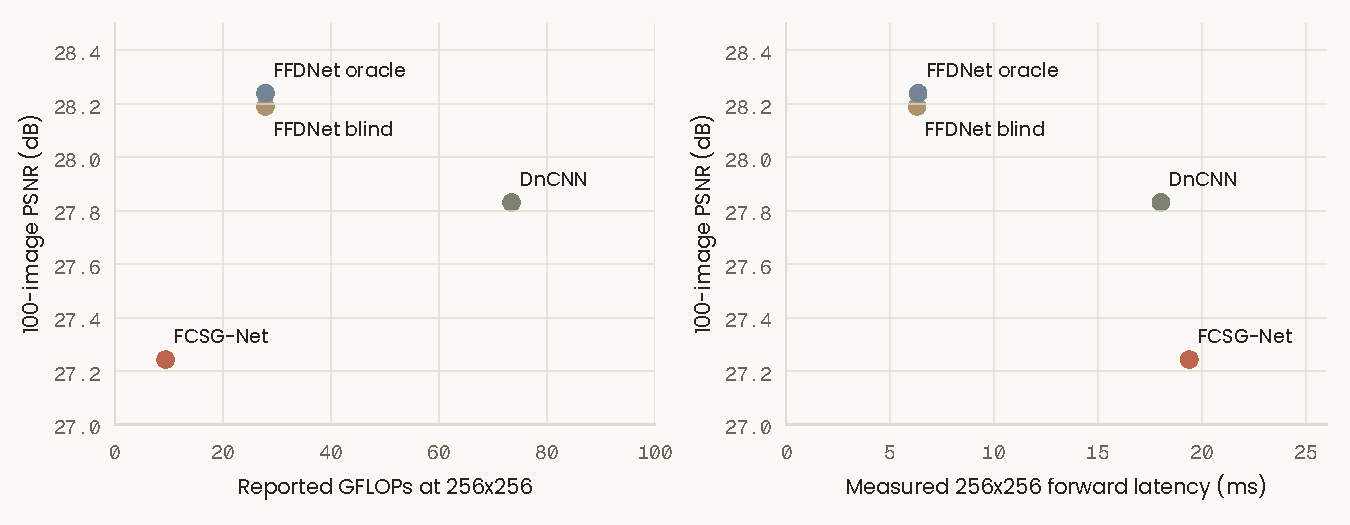
\includegraphics[width=0.95\linewidth]{compute_latency.pdf}
	\caption{Validation PSNR against reported GFLOPs (left) and against
	measured $256\times256$ latency (right).}
	\label{fig:cost}
\end{figure}

\section{Routing analysis}\label{sec:routing}

We studied the final \fcsg{} checkpoint on ten validation images, each
degraded with eight seeds. That gives 80 samples from ten independent images.

\paragraph{Where the gate routes.} The dense routing probabilities end up
close to uniform, with a mean entropy of 1.09 to 1.10 nats per band against a
maximum of 1.10. Taken alone, that suggests the gate learned nothing. The
top-2 selection says otherwise. In the high band the gate picks the
$3\times3$ expert at 99.98\% of pixels, and the larger experts share the
second slot depending on location. The maps follow image structure
(Figure~\ref{fig:routing-map}). Top-2 selection flips when two logits swap
rank, so near-uniform probabilities can still produce a sharp, consistent
choice.

\begin{figure}[htbp]
	\centering
	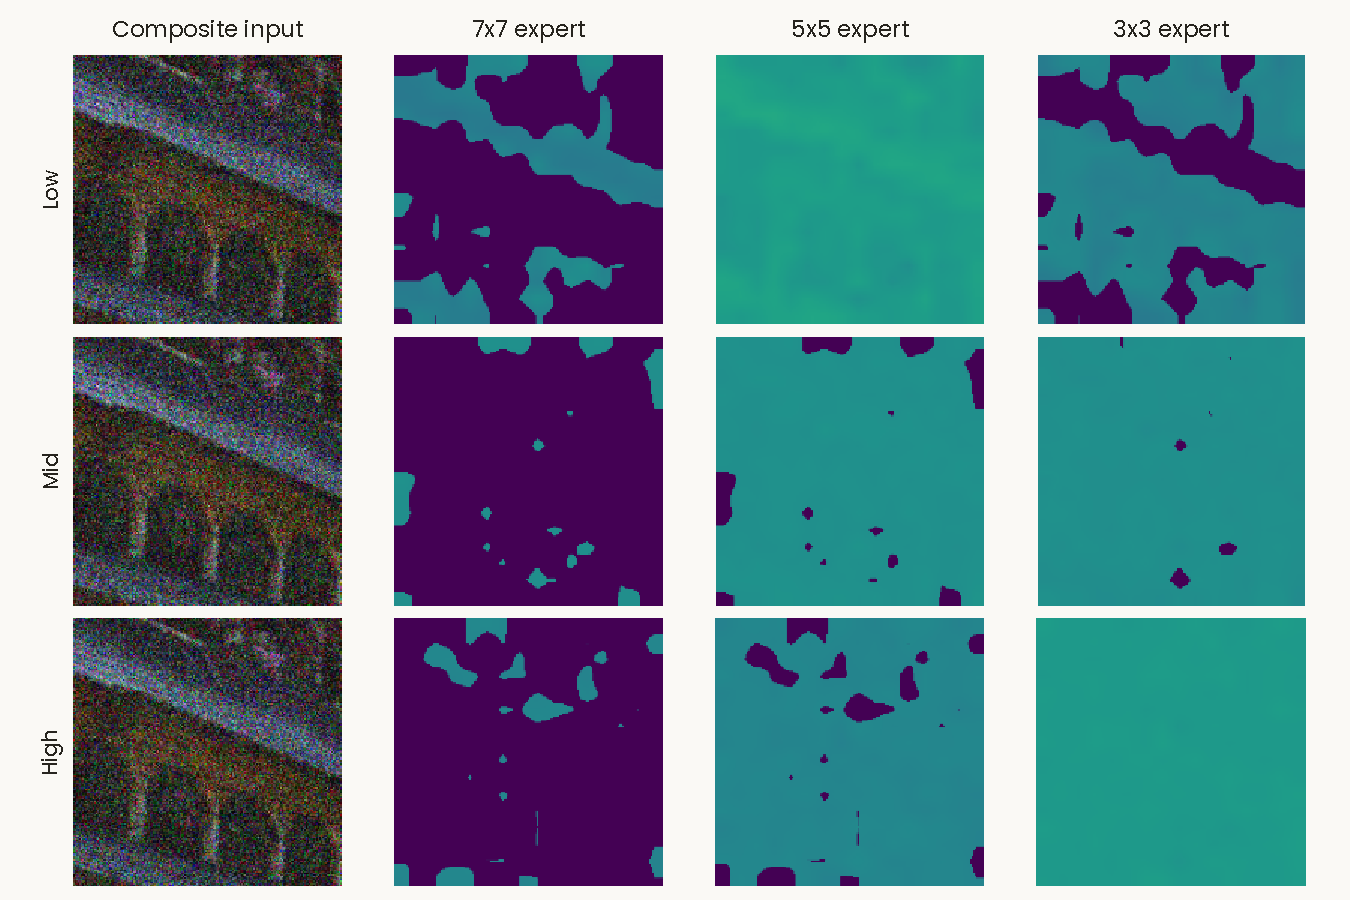
\includegraphics[width=0.9\linewidth]{routing_0834.pdf}
	\caption{Expert weights for validation image 0834. Rows show the low, mid
	and high band. Columns show the degraded crop and the weights of the
	$7\times7$, $5\times5$ and $3\times3$ experts.}
	\label{fig:routing-map}
\end{figure}

\paragraph{Routing and the degradation.} After subtracting each image's
mean, the high-band $3\times3$ weight correlates at $r=+0.81$ with the noise
level. The low-band $5\times5$ weight correlates at $+0.80$ and the low-band
$7\times7$ weight at $-0.73$. More noise moves weight toward smaller kernels.
All six of the strongest correlations involve noise. The strongest with blur
is $+0.42$ and the strongest with JPEG quality is $-0.39$. These results are
exploratory. They come from ten images and 36 correlations with no
multiple-comparison correction, and the four parameters move together. They
show a consistent response, not a causal one.

\paragraph{Does the model need the gate?} We kept the trained weights and
overrode the gate at inference. Table~\ref{tab:interventions} gives the
result.

\begin{table}[htbp]
	\centering
	\caption{PSNR change when we override the trained gate at inference (10 images).}
	\label{tab:interventions}
	\small
	\begin{tabular}{@{}lrr@{}}
		\toprule
		Intervention & Mean $\Delta$PSNR & Min / max \\
		\midrule
		Equal weights on the selected pair     & $-0.040$\dB & $-0.137$ / $+0.028$ \\
		Uniform weights over all three experts & $-0.372$\dB & $-0.986$ / $+0.163$ \\
		\bottomrule
	\end{tabular}
\end{table}

Flattening the weights inside the chosen pair barely matters. Dropping the
choice itself costs 0.37\dB{} on average and nearly 1\dB{} on one image. The
trained network cares far more about \emph{which} experts are combined than
about how they are weighted. So the gate does real work in this model.
Whether a model trained without a gate would do worse is a separate question
that needs a matched training ablation, which we leave to future work.

\section{Discussion}\label{sec:discussion}

The routing works in the sense we set out to test. It varies across the
image, follows the noise level and matters to the trained model. It does not
make the model competitive. With under 100,000 parameters, \fcsg{} trails
baselines six to nine times its size by 0.6 to 1.0\dB{}, most likely for lack
of capacity, and it is no faster on a GPU. Frequency-band routing is a cheap
way to make a small model's behaviour visible. Within our budget, it does not
on its own make the model better or faster.

\chapter{Conclusion and future work}\label{ch:conclusion}

\section{Conclusion}\label{sec:summary}

\fcsg{} splits an image into three frequency bands and routes each band, per
pixel, to two of three shared convolutional experts. With 97,088 parameters
and 9.39 GFLOPs, it passed every check before training (O1). Our FFDNet code
matched the published CBSD68 result to within 0.01\dB{} (O2). Under one
matched composite-degradation protocol, \fcsg{} reached 27.24\dB{}. That is
0.59\dB{} below DnCNN and 0.95\dB{} below blind FFDNet, with 82.6\% and
88.6\% fewer parameters. It was also the slowest model on a Tesla T4 (O3).
Its gate varies across the image and follows the noise level, with
correlations up to 0.81. The trained model loses 0.37\dB{} when we override
the gate's choices (O4). Frequency-band routing gave a small model behaviour
we can inspect. It did not beat simple baselines on accuracy or speed.

\section{Limitations}\label{sec:limitations}

We trained each model once, and all results come from the validation split,
with no untouched test set. The degradation is synthetic. We did not test on
real archival photographs or run a human study. The routing analysis rests on
ten images and exploratory correlations. The interventions measure how much
the trained model leans on its gate, not what a gate adds during training. We
measured latency on one GPU without an operator profile. Every expert always
runs, so sparse routing saves no computation.

\section{Future work}\label{sec:future}

The first experiment to run is a matched training ablation. It would compare
learned routing with fixed uniform weights, from the same initialisation and
with several seeds. Further ablations would test the kernel sizes, a
per-image gate, plain concatenation in place of SE fusion, and hard masks.
The model relies mainly on which experts it picks, so skipping unselected
experts could save up to a third of the expert cost. An operator profile
should come first, along with latency measurements on CPU and mobile
hardware. The parameter budget is fifty times what the model uses, so
widening the experts could close the capacity gap, provided cheaper expert
evaluation frees up compute. Last, any claim about archival restoration needs
real archival images, a controlled degradation sweep and a held-out test set.

\cleardoublepage

% ---------------------------------------------------------------- back matter
\rhead{\textit{References}}
\lhead{}
\renewcommand\bibname{References}
\bibliographystyle{Ref/IEEEtran}   % CS/EE norm; the template lists it as an option
{
	\fontsize{10}{12}
	\selectfont
	\addcontentsline{toc}{chapter}{References}
	\bibliography{Ref/references}
}
\cleardoublepage

% Dissemination: keep only if a paper/poster/preprint exists. Otherwise delete.
%\rhead{\textit{Dissemination}}
%\lhead{}
%\input{Ref/Dissemination}
%\thispagestyle{empty}
%\cleardoublepage

% Index: the template ends with \indexColumns{3}\indexPage. It is only useful
% if someone tags terms with \index{...} while writing. Drop it otherwise.
%\indexColumns{3}
%\indexPage
\end{document}
